\documentclass[UTF8]{article} 
\usepackage{graphicx}
\usepackage{subfigure}
\usepackage{amsmath}
\usepackage{makecell}
\usepackage[utf8]{inputenc}
\usepackage[space]{ctex} %中文包
\usepackage{listings} %放代码
\usepackage{xcolor} %代码着色宏包
\usepackage{CJK} %显示中文宏包
\usepackage{float}


\definecolor{mygreen}{rgb}{0,0.6,0}
\definecolor{mygray}{rgb}{0.5,0.5,0.5}
\definecolor{mymauve}{rgb}{0.58,0,0.82}
\lstset{
	backgroundcolor=\color{white}, 
	%\tiny < \scriptsize < \footnotesize < \small < \normalsize
	basicstyle = \scriptsize,
	breakatwhitespace = false,        
	breaklines = true,                 
	captionpos = b,                    
	commentstyle = \color{black}\bfseries,
	extendedchars = false,             
	frame =shadowbox, 
	framerule=0.5pt,
	keepspaces=true,
	keywordstyle=\color{black}\bfseries, % keyword style
	language = C++,                     % the language of code
	otherkeywords={string}, 
	numbers=left, 
	numbersep=5pt,
	numberstyle=\tiny\color{black},
	rulecolor=\color{black},         
	showspaces=false,  
	showstringspaces=false, 
	showtabs=false,    
	stepnumber=1,         
	stringstyle=\color{black},        % string literal style
	tabsize=4,          
	title=\lstname                      
}
\newcommand{\jumpLine} {\hspace*{\fill} \par}
\newcommand{\keypoint}[1]{$\bullet$\quad#1\par}
\newcommand{\keypointt}[2]{$\bullet$\textbf{#1}\quad#2\par}


\title{中国科学技术大学计算机学院\\《计算机系统概论》实验报告}
\author{}

\date{}

\begin{document}
	\maketitle
	\begin{figure}[H]
		\centering
		
\includegraphics[width=2.5in]{xiaohui.jpg}\vspace{0.5cm}\\
		\large{
			实验题目:两正数的最大公因数\\
			学生姓名:王章瀚\\
			学生学号:PB18111697\\
			完成日期:\today\\
		}\vspace{2cm}
		
		\large{计算机实验教学中心制\\2019年09月\\}
		\thispagestyle{empty}
		\clearpage  % 清除当页页码
	\end{figure}


	\section{实验要求}
	\subsection{总述}
	用LC-3汇编语言写一个程序,并编译成obj文件。这个程序用以计算两个正数的最大公因数。
	\subsection{细节要求}
	\keypoint{两个正数以16-bit有符号数给出,存在R0和R1两个寄存器.输出应置于R0.}
	\keypoint{不要使用除了x3000-xFDFF的内存空间.}
	\keypoint{程序结尾应是HALT.}
	\keypoint{R7应该保持不变.}
	
	
	\section{设计思路}
	\subsection{总述}
	要求最大公因数,必然能想到的是辗转相除法或更相减损术。然而在LC-3中,并没有除法可供直接使用,因为其没有直接的硬件上实现。因此即便想用辗转相除法的思路,也将在LC-3中退化为更相减损术。\par
	诚然,存在其他一些方法,比如逐一检验法(从最小的一个数开始逐个到1地检验是不是公因子)或取素因数分解指数最小值。这些方法可能在高级语言中看上去会比较优美,但在LC-3这样一个RISC指令集中,似乎并不那么适用。\par
	综上所述,本次实验,将使用更相减损术的思路来完成。下面具体阐述算法。\par
	\subsection{初步思路}
	既然使用更相减损术,则相互做减法运算即可。\par
	以下是算法流程图。R0,R1为相减过程中的数,R2用以计算-R1。\par
	\begin{figure}[H]
		\centering
		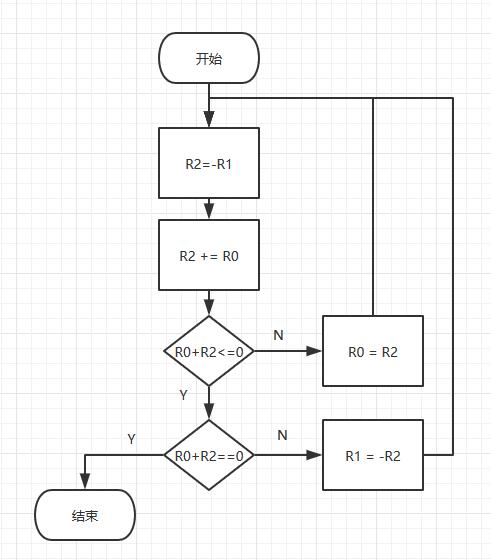
\includegraphics[width=0.6\linewidth]{process1.jpg}
		\caption{初步思路的流程图}
		\label{process1}
	\end{figure}\par
	至于其具体代码,下面将会讲解。\par

	\subsection{改进思路}
	上面的初步思路有个很大的缺点,就是当一个数远大于另一个数的时候,需要做多次减法,但每一次都重新计算了同一个数的相反数,这使用的指令数是比较多的。\par
	以下是一个优化的办法:不妨设R0远大于R1,则令R3=R0-R1,然后循环这条指令"R3=R3-R1",直到R3<0,这时只需要将R0赋值为R3+R1即可。另一种情况同理。这样子就免去了多次计算的麻烦。\par
	以下是这种思路的流程图,为了简洁起见,减法运算直接表示出来,而不是用“取反加一”来表示。\par
	
	\begin{figure}[H]
		\centering
		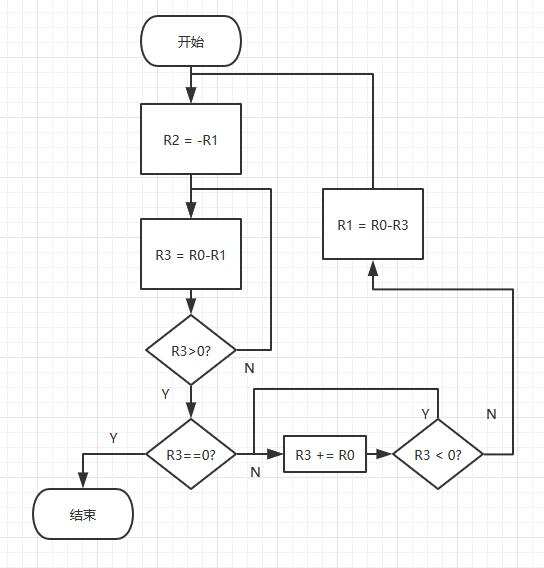
\includegraphics[width=0.6\linewidth]{process2.jpg}
		\caption{改进思路的流程图}
		\label{process2}
	\end{figure}\par
	至于其具体代码,下面将会讲解。\par
	
	\subsection{另一个思路:结合查找表}
	除了上述的改进办法以外,还有一些其他的想法。例如,可以用查找表来实现右移,以此能够较好地避免两数相差多大需要多减很多次。\par
	这一步改进的主要思路可以由下面流程图体现:\par
	\begin{figure}[H]
		\centering
		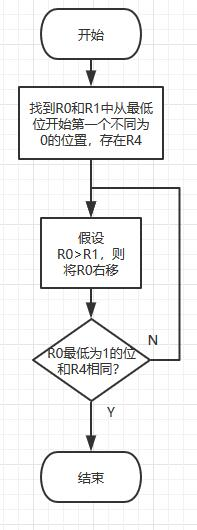
\includegraphics[width=0.3\linewidth]{process3.jpg}
		\caption{结合查找表右移的方法}
		\label{process3}
	\end{figure}\par
	而查找表中,将第14位单独判断,后面几位利用x8000以后的x8000个内存空间来直接查找获得。表的部分如下:\par
	\jumpLine
	\begin{tabular}{|c|c|}
		\hline 
		x4000 & x0000 \\ 
		\hline 
		x4001 & x0000 \\ 
		\hline 
		x4002 & x0001 \\ 
		\hline 
		x4003 & x0001 \\ 
		\hline 
		x4004 & x0002 \\ 
		\hline 
		... &  ... \\ 
		\hline 
	\end{tabular} \par
	该方法的一个示例如下:\par
	\begin{tabular}{|c|c|c|}
		\hline 
		步骤 & R0 & R1 \\ 
		\hline 
		0 & 1100 & 0010 \\ 
		\hline 
		1.1 & 0110 & 0010 \\ 
		\hline 
		1.2 & 0100 & 0010 \\ 
		\hline 
		2.1 & 0010 & 0010 \\ 
		\hline 
		2.2 & 0000 & 0010 \\ 
		\hline 
	\end{tabular} 
	
	
	\section{时空复杂度分析}
	\subsection{初步思路}
	对于初步思路,使用更相减损术。\par
	空间复杂度上,使用了三个寄存器,为o(3)~o(1)。\par
	时间复杂度上,最好的情况就是两数相等,此时时间复杂度为o(1);而最坏的情况中,有一种是一个数为1,另一个数为a时,复杂度为o(a)。可想而知,若两个数为a,b。则相减次数必然不超过max\{a,b\}就可以减到1。综合这两点可以看出来,其时间复杂度最坏为o(max\{a, b\})
	\subsection{改进思路}
	对于改进了的思路,多使用了一个寄存器。\par
	空间复杂度应为o(4)~o(1)。\par
	时间复杂度上,由于改进处在于减少了取相反数的次数。因此就复杂度而言仍然是o(max\{a, b\})的。只不过每一个循环主体少执行了一些语句。\par
	\subsection{结合查找表}
	由于加了查找表,多用了x8000个地址,故其空间复杂度为o(x8000),而时间复杂度上,假设为a, b两数。且a末尾0比b多n个,则时间复杂度至多为$o(max\{\frac{a}{2^{n}}, b\})$。\par
	
	
	\section{关键代码讲解}
	\subsection{初步思路}
	初步思路的代码实现如下:\par
	\begin{lstlisting}[language=C++, name=初步思路的代码]
			.ORIG	x3000
	
	LOOP	NOT	R2, R1
			ADD	R2, R2, #1
			ADD	R2, R0, R2	
			BRnz	NZ		;R0>R1
			ADD	R0, R2, #0
			BRnzp	LOOP
	NZ		BRn	N			;R0<R1
			BRnzp	OK		;R0==R1
	N		ADD	R2, R2, #-1
			NOT	R2, R2
			ADD	R1, R2, #0
			BRnzp	LOOP
		
	OK		HALT
			
			.END
	\end{lstlisting}
	按照上述思路,对R0>R1, R0==R1, R0<R1三种情况进行分类处理,代码十分简洁,相应注释已写上,故不再赘述其内容。\par
	
	\subsection{改进思路}
	改进思路的代码实现如下:\par
	\begin{lstlisting}[language=C++, name=改进思路的代码]
			.ORIG	x3000
	
	LOOP	NOT	R2, R1
			ADD	R2, R2, #1
			ADD	R3, R0, R2
			BRnz	NZ		;R0 > R1
	P		ADD	R3, R3, R2	;减减看
			BRp	P			;是正数则减到非正
			ADD	R0, R1, R3	;更新R0为R1+R3
			BRnzp	LOOP
	NZ		BRn	N		
			BRnzp	OK		;R0==R1,结束
	N		ADD	R3, R3, R0	;否则R0<R1,加加看
			BRn	N			;是负数则加到非负
			NOT	R3, R3
			ADD	R3, R3, #1
			ADD	R1, R0, R3	;更新R1为R0-R3
			BRnzp	LOOP
			
	OK		HALT
			
			.END
	\end{lstlisting}
	在该代码中,标签P表示的部分是对R0>R1的情况的处理,N部分表示的是R0<R1的情况处理。代码相对清晰,注释也较为完善,可根据注释和上述流程图较好地理解程序。\par
	
	
	\subsection{另一个思路:结合查找表}
	\begin{lstlisting}[language=C++, name=改进思路的代码]
			.ORIG	x3000
	
	; 测试需要移位到哪
	RSHIFT		NOT 	R2, R0
				NOT		R3, R1
				LD		R4, DEC1
				AND		R5, R2, R3
	NEXT_TEST	AND		R6, R5, R4
				BRz		DO
				ADD		R4, R4, R4
				BRnzp	NEXT_TEST
	
	; 移位开始前的一些准备
	DO			LD		R2, HEX4000
				AND		R5, R0, R4
				BRz		R0_RSHIFT	
	
	; 对R1右移
	R1_RSHIFT	ADD		R3, R1, R2
				LDR		R1, R3, #0
				AND		R5, R1, R4	;确认是否移到
				BRz		R1_RSHIFT
				BRnzp	MINUS
	
	; 对R0右移
	R0_RSHIFT	ADD		R3, R0, R2
				LDR		R0, R3, #0
				AND		R5, R0, R4	;确认是否移到
				BRz		R0_RSHIFT	
	
	; 更相减损术
	MINUS		NOT		R3, R1
				ADD		R3, R3, #1
				ADD		R3, R0, R3
				BRn		MINUS_TO_N
				BRz		OK
				ADD		R0, R3, #0
				BRnzp	RSHIFT
	MINUS_TO_N	ADD		R3, R3, #-1
				NOT		R3, R3
				ADD		R1, R3, #0
				BRnzp	RSHIFT
	
	OK			HALT
	
	DATA_LOC	.FILL	xD000
	
	LUT			.FILL	x4000
	DEC1		.FILL	#1
	HEX4000		.FILL	x4000
	.END
	\end{lstlisting}
	
	
	\section{调试分析}
	\subsection{平均指令数}
	为了检验改进是否有效,用C语言生成了10000个随机数来测试,结果如下:
	\begin{figure}[H]
		\begin{minipage}[H]{0.33\linewidth}
			\centering
			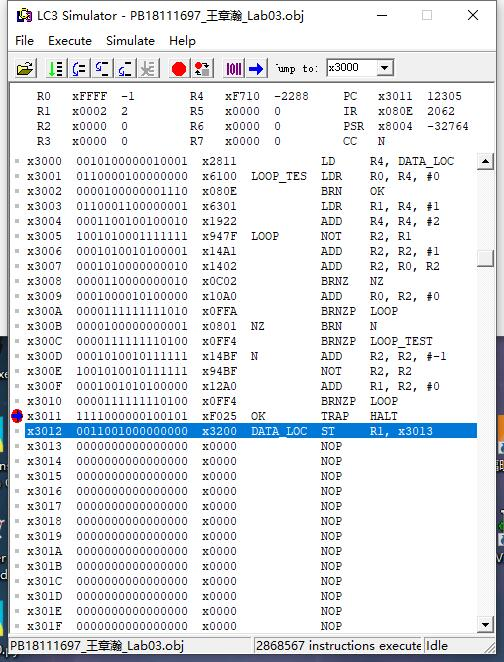
\includegraphics[scale=0.33]{data0_1.jpg}
			\caption{10000个随机数测试——初步思路(平均指令数2868567/5000=574条)}
			\label{data0_1}
		\end{minipage}
		\qquad
		\begin{minipage}[H]{0.33\linewidth}
			\centering
			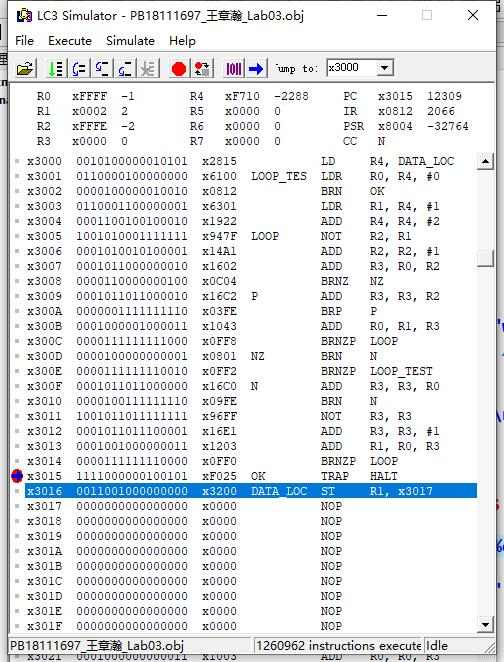
\includegraphics[scale=0.33]{data0_2.jpg}
			\caption{10000个随机数测试——改进思路(平均指令数1260962/5000=252条)}
			\label{data0_2}
		\end{minipage}
		\begin{minipage}[H]{0.33\linewidth}
			\centering
			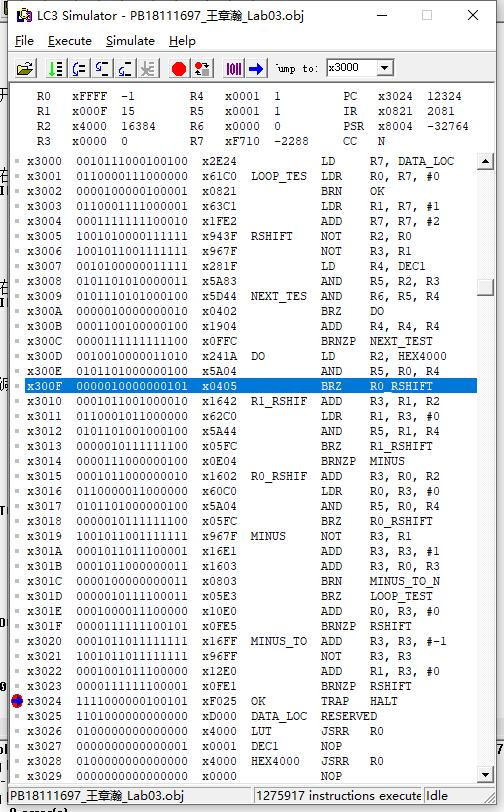
\includegraphics[scale=0.33]{data0_3.jpg}
			\caption{10000个随机数测试——结合查找表(平均指令数1275917/5000=255条)}
			\label{data0_3}
		\end{minipage}
	\end{figure}
	可以看出来,改进后的方式的平均指令数为改进前的$\frac{2}{5}$左右。确实是很大的进步。而结合查找表和改进思路不相上下。\par
	注:上面截图中R0均为-1,是因为设置了-1作为哨兵来确认是否使用了所有数据。并不是求出了最大公因数为-1。\par
	
	
	\subsection{特殊测试数据选取}
	对于此题的测试数据选取,有三个极端值得一看考虑。\par
	\subsubsection{测试数据1}
	一种应该选取两数之比接近$\frac{\sqrt{5}+1}{2}$的值,如1618和1000。这能将改良算法的优化降低至接近0甚至比原来差。这个值的推导过程大致如下表:\par
	\begin{tabular}{|c|c|c|c|c|c|}
		\hline 
		R0 & x & x-y & x-y & 2x-3y & ... \\ 
		\hline 
		R1 & y & y & 2y-x & 2y-x & ... \\ 
		\hline 
		另一寄存器改值的条件 & x>y & 2y>x & $x>\frac{3}{2}y$ & $\frac{5}{3}y>x$ & ... \\ 
		\hline 
	\end{tabular} \par
	最后会得到x和y的比例应该是$\frac{\sqrt{5}+1}{2}$左右。\par
	测试结果如下:\par
	\begin{figure}[H]
		\begin{minipage}[H]{0.48\linewidth}
			\centering
			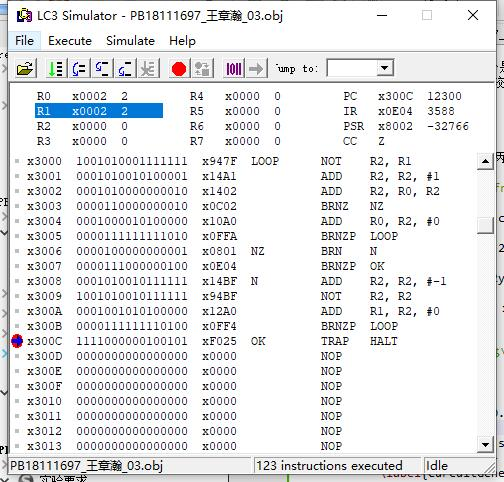
\includegraphics[scale=0.45]{data1_1.jpg}
			\caption{测试数据1——初步思路(123条指令)}
			\label{data1_1}
		\end{minipage}
		\qquad
		\begin{minipage}[H]{0.48\linewidth}
			\centering
			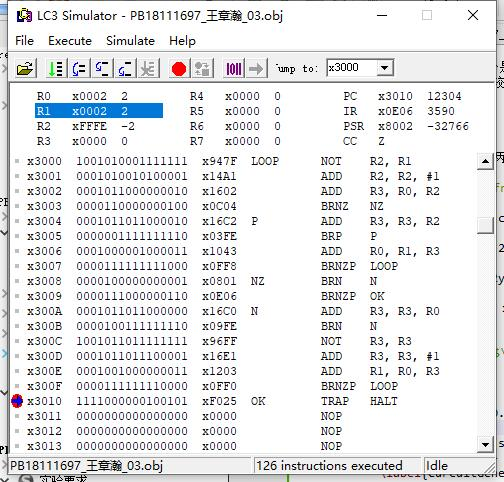
\includegraphics[scale=0.45]{data1_2.jpg}
			\caption{测试数据1——改进思路(126条指令)}
			\label{data1_2}
		\end{minipage}
	\end{figure}

	\subsubsection{测试数据2}
	另一种则是前面提到的一个是1,另一个是n。为了表现出其极端性,取1和x0FFF。\par
	测试结果如下:\par
	\begin{figure}[H]
		\begin{minipage}[H]{0.48\linewidth}
			\centering
			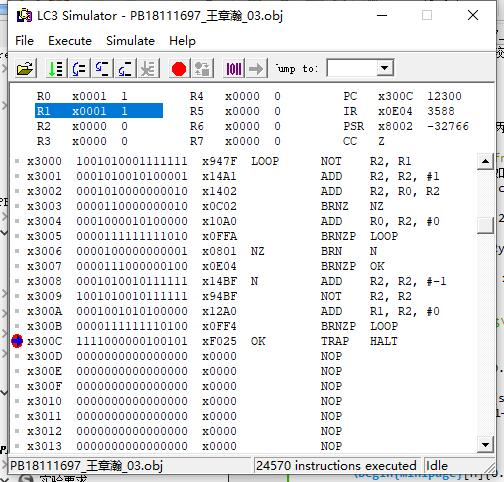
\includegraphics[scale=0.45]{data2_1.jpg}
			\caption{测试数据2——初步思路(24570条指令)}
			\label{data2_1}
		\end{minipage}
		\qquad
		\begin{minipage}[H]{0.48\linewidth}
			\centering
			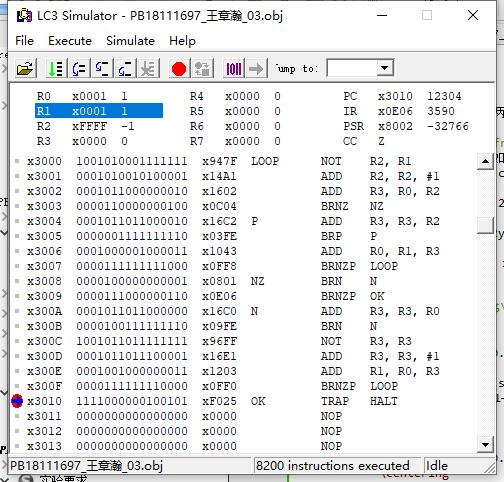
\includegraphics[scale=0.45]{data2_2.jpg}
			\caption{测试数据2——改进思路(8200条指令)}
			\label{data2_2}
		\end{minipage}
	\end{figure}

	\subsubsection{测试数据3}
	另一种则是为了对比查找表方法和改进思路方法。取x7000和x0001。则有如下运行结果:\par
	\begin{figure}[H]
		\begin{minipage}[H]{0.48\linewidth}
			\centering
			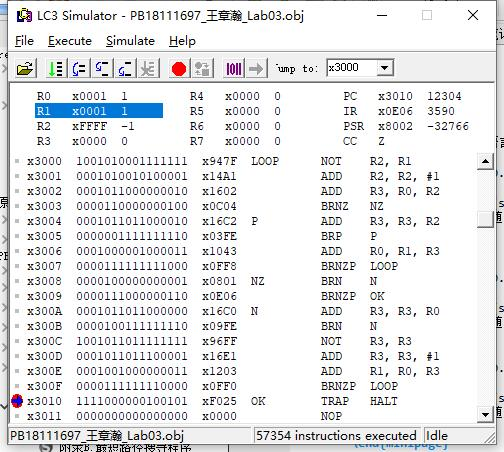
\includegraphics[scale=0.45]{data3_2.jpg}
			\caption{测试数据2——初步思路(57354条指令)}
			\label{data3_2}
		\end{minipage}
		\qquad
		\begin{minipage}[H]{0.48\linewidth}
			\centering
			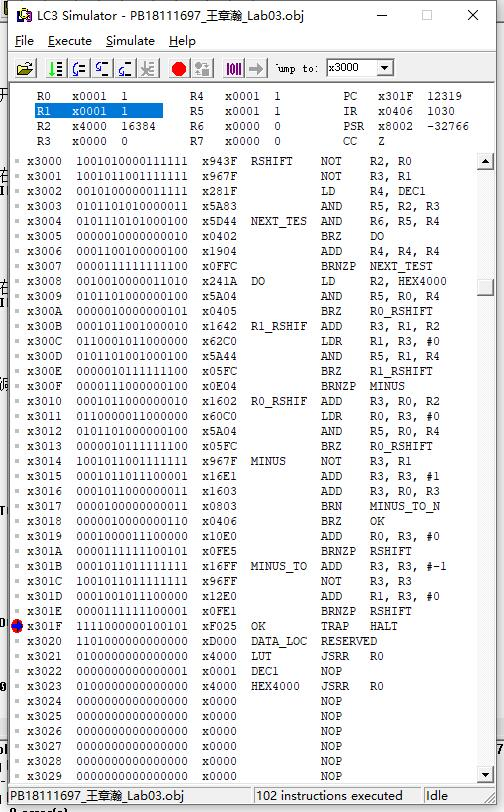
\includegraphics[scale=0.45]{data3_3.jpg}
			\caption{测试数据2——结合查找表思路(102条指令)}
			\label{data3_3}
		\end{minipage}
	\end{figure}
	可以明显看出,但两个数的末尾0数量差的比较多的时候,借助查找表执行右移将大大提升效率。
	
	
	
	\subsection{对测试结果的评述}
	可以看出来,对改进算法最不利的时候,多使用的语句数也并不多很多。然而对初步思路最不利的时候,改进思路的提升就很显然了。\par
	而对于查找表右移的方法,最佳情况是两个数的末尾0个数差的比较多,可以快速右移而不是一个一个慢慢地减。\par

	\section{对负数和零的处理}
	如果是负数,可以一开始就检测正负性,将负数改为正数即可。如果是0,则直接将R0置为另一个数的绝对值。这都是十分简单的处理。\par
	
	
	\section{Great Idea}
	\keypointt{更相减损术中的求相反数}{由于可能要用到多次这个相反数,于是将得到的相反数重复利用直到不可再用。}
	\keypointt{查找表的使用}{由于第三个思路需要用到右移的操作。而从上一次实验可以知道,常规右移需要的指令数是极大的,因此如果能借用查找表,将会使得指令数只需要一到两条。大大减少了右移的损耗。}
	
	\section{实验总结}
	本实验在LC-3中实现了更相减损术。可以看出来,对于LC-3这样的精简指令集体系结构,我们难以使用除法这样的计算;此外,如果能够重复利用的数据一定要重复利用,尽量避免重新计算带来的对执行指令数的大幅增加。\par
	此外,查找表也是一种很好的方法,它能够避免一些难以实现的运算从而以空间换时间来完成想要的功能。\par
	最后说明,由于查找表不容易让助教批改,故提交的是改进思路的代码。\par
	
	
	
	
	
	
\end{document}
